\documentclass[journal]{IEEEtran}

\usepackage{biblatex}

\usepackage[fleqn]{amsmath}
\usepackage{amssymb}
\usepackage{graphicx}
\usepackage{cancel}
\addbibresource{./citations.bib}

% \graphicspath{ {C:/Users/jonat/Documents/ECH-267-Adv.-Proc.-Control/Project/1_Report/images/}}
\graphicspath{ {C:/Users/Indy-Windows/Documents/ECH-267-Adv.-Proc.-Control/Project/1_Report/images/}}

\usepackage{hyperref}
\hypersetup{
colorlinks=false,
linkcolor=blue,
filecolor=magenta,
    urlcolor=blue,
}
\urlstyle{same}

% \hyphenation{op-tical net-works semi-conduc-tor}


\begin{document}

\title{MPC for Robotic Arm Path Planning and Control \\ ECH-267 Final Project Report}


\author{Jonathan~Dorsey \IEEEmembership{Member: No Sleep Club: est. 2017} \\  \url{https://github.com/JonnyD1117/ECH-267-Adv.-Proc.-Control/tree/main/Project}}


% The paper headers
\markboth{Journal of Graduate School Assignments, March~2021}%
{Dorsey \MakeLowercase{\textit{et al.}}: MPC for Robotic Arm Path Planning and Control ECH-267 Final Project Report}

% make the title area
\maketitle

% As a general rule, do not put math, special symbols or citations
% in the abstract or keywords.
\begin{abstract}
  The objective of this project is to implement a simulated optimal \underline{Path Planner} using Model Predictive Control (MPC) to plan and control the behavior of a 2 degree of freedom (2DOF) robotic arm. The responsibility of the MPC planner will be to generate the `optimal' path and to drive the arm from its current position to the next. The main challenges faced in completing this project consist of solving for the \textbf{nonlinear equations of motion} (as well as any required forward/inverse kinematics) of the robotic arm as well as formulating and solving the \textbf{MPC controller}, at each timestep, both control and planning using the CasADi optimization framework, to test the scenario of simulated real-time performance.
\end{abstract}

% Note that keywords are not normally used for peerreview papers.
\begin{IEEEkeywords}
Model Predictive Control, Robot Arm, Lagrange Equations, Path Planning, Obsticle Avoidance, DH Parameters, Trajectory Generation.
\end{IEEEkeywords}


\IEEEpeerreviewmaketitle

\section{Introduction}

\IEEEPARstart{T}{he} world of robotics is full of constraints, demands, and performance trade-offs that humans handle naturally on a daily basis. Unlike humans, robots require control and planning strategies which are flexibility enough to work around constraints and limitations, while accurately meeting control and performance objectives in uncertain environments. While the emergence of machine learning techniques and methods offers promise of stateoftheart improvements and performance, most robotic systems still demand a more practical and robust planning and control algorithms, capable of offering a compromise between the performance criteria, flexibility to navigate constraints, and amount of computational power required to compute valid control commands in real-time. \\

In the world of robot manipulators, tasks can range from relatively simple and coarse motions to extremely complex and detailed actions. One common control strategy which has seen great success, in robotics, in recent years is Model Predictive Control (MPC). MPC is an optimal control methodology which solves the a given optimal control problem (OCP) in a receding fashion, over a finite horizon. While these controllers are far more sophisticated than standard classical or modern control strategies, the increased complexity and computation can be applied to a wider class of control problems. This flexibility in natively handling constraints as well as naturally extending to nonlinear and multiple-input-multiple-output-systems makes MPC an attractive candidate control methodology for the vast world of robotics where tasks can range from autonomous mobile vehicles to robotic manipulators. While MPC has the obvious conns of requiring an approximate solution to an optimization problem, at each time step, the benefits which this methodology offers often make it a viable solution even with the added computationally expense. \\

While control is an important aspect of modern robotics, it is often more valuable to have an understanding of the intent or future actions which an autonomous system believes it should take, to accomplish a goal. In general, this problem is known as \textbf{path planning}, and is an important part of modern robotics research. Many modern path planning approaches use a vast array of different planning paradigms, such as discretization, graph, probablistic, and heuristic methods which have all shown great promise, and present there own unique benefits and limitations. Often in the more general case of motion planning, it is desirable to not only control the position, but also the velocity and acceleration of a system, in both space and time. However, for the purpose of this paper, only the more restricted case of path planning (e.g. position planning) will be considered.  \\

To this point, another possible method for path planning is the use of MPC, as a optimal path planner. MPC has the potential to provide much of the same functionality as other planning strategies by implementing desireable behavior into a cost function or functional constraints. The ability to leverage and model predictive controller as a path planning with practically no changes to its implementation as a controller also offers an opportunity for systems using MPC to obtain some path planning capabilities for free.   \\

While MPC has been received enormous amounts of research across many fields, including  robotics, many of the applications in robotics focus MPC on mobile robotics such as drones and autonomous vehicles, with significantly less attention focused on the application of MPC as a controller or a planner for robotic manipulators.

\section{Problem Statement}

This paper will investigate the use of MPC as a general control scheme and its utility as a path planner for a simple two link planar robotic manipulator. By the use of simulation, this paper will develop and identify key elements in understanding some of the benefits and limitations of MPC in the context of articulated robotic manipulators.

\subsection{Planar RR Robotic Arm}

The manipulator used in this paper is a two link planar robot arm subject to gravity, fig.\ref{RRrobot}, commonly known as a \textbf{RR} (revolute-revolute) robot. This model commonly does not include any rigid body dynamics and treats the robot as a system of point masses directly coupled with massless rods. While this configuration is very simple, it is conceptually simple, easy to derive its core dynamics, and facilitates a more focused study on the planning and control elements of the paper.

\begin{figure}
    \centering
    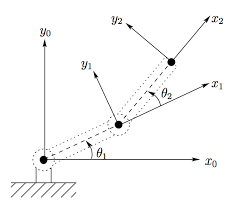
\includegraphics[scale=.5]{2d_arm_2}
    \caption{RR Planar Manipulator subject to gravity}
    \label{RRrobot}
\end{figure}

% \subsection{MPC Control Objectives}
% From a strictly control perspective, this paper seeks to investigate how to formulate MPC for the robot arm, to determine the effectiveness of MPC in , to
%
%
%
% for as a
%
% \begin{enumerate}
%     \item How can MPC be used to control a simple robot?
%     \item How effective is MPC over other control schemes?
%     \item Can MPC be used for obstacle avoidance?
%     \item How long does it take MPC to generate a solution for each time step
% \end{enumerate}
%
% \subsection{Path Planning Objectives}
%
% \begin{enumerate}
%     \item How can MPC be used as a simple path planner
%     \item how reliable is form of path planner
%     \item Can this planner be used reference for
%     \item What restriction on the performance of the sytem does using using this path planner enforce
% \end{enumerate}
%
%
%
%
%
%
% to performance of standard Multiple Shooting MPC on simplified robotic manipulator, quantify the computational burden of implementing MPC, test the flexibility MPC as a framework for advanced control objectives (obstacle avoidance), and to


\section{Background}

To contextualize the implementation of MPC for on robotic manipulators, it is helpful to breakdown a few of the fundamental elements, constructs, and terminology which are commonly used in robotics literature.

\subsection{Robotic Manipulators}

In general robotic arms are classified as either prismatic (linear motion) or revolute (rotational motion) joints. The PUMA 560 [Fig.\ref{puma560}], is an industry standard 6 degree of freedom (DOF) manipulator. It utilizes six revolute joints, connected in a serial fashion. This configuration of only rotating joints makes the PUMA 560 an \textbf{articulated robot}.

\begin{figure}
    \centering
    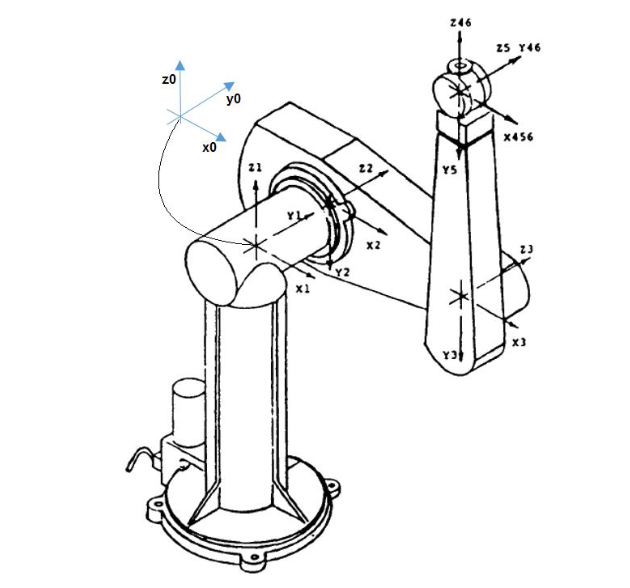
\includegraphics[scale=.5]{puma}
    \caption{Puma560 Robot with Joint Coordinate Frames}
    \label{puma560}
\end{figure}

While the study of high DOF robots is well researched and would be present interesting and complicated scenarios for both control and planning, the scale and complexity of modeling the governing dynamic equations make robots like those in [Fig. \ref{puma560}] impractical for the scope and time restrictions of this paper. This paper, instead, opts to use the dynamically simple RR-robot described above, as its design and test platform for implementing MPC.



\subsubsection{DH Parameters \& Homogenous Transforms}

The Denavit-Hartenberg (DH) parameters are an important tool in describing the geometry of any given robot, and prove to be highly effective in the formulation of joint transformations which enable a concise and universal method for transforming important quanties for kinematic and dynamic analysis of a robot.\\

\noindent The DH Parameters are defined to be...
    $$
    \begin{array}{l}
    a_{i}=\text { the distance from } \hat{Z}_{i} \text { to } \hat{Z}_{i+1} \text { measured along } \hat{X}_{i} \\
    \alpha_{i}=\text { the angle from } \hat{Z}_{i} \text { to } \hat{Z}_{i+1} \text { measured about } \hat{X}_{i} \\
    d_{i}=\text { the distance from } \hat{X}_{i-1} \text { to } \hat{X}_{i} \text { measured along } \hat{Z}_{i} ; \text { and } \\
    \theta_{i}=\text { the angle from } \hat{X}_{i-1} \text { to } \hat{X}_{i} \text { measured about } \hat{Z}_{i}
    \end{array}
    $$


By utilizing the \textbf{homogeneous transform}, which describes the frame position and rotation required to define a vector from one frame to another, we generate a mapping of a vector to or from any coordinate system in the system.

\begin{equation}
    $$
    \left[\begin{array}{c}
    {}^{A}P \\
    1
    \end{array}\right]=\left[\begin{array}{ccc|c}
    {} & {}^{A}_{B}R & & {}^{A}P_{B org} \\
    \hline 0 & 0 & 0 & 1
    \end{array}\right]\left[\begin{array}{c}
    {}^{B}P \\
    1
    \end{array}\right]
    $$
\end{equation}


\begin{equation}
        P = { }_{B}^{A} T^{B} P
\end{equation}

DH parameters can be used to define a single transformation from frame $\{ i\}$ to frame $\{ i-1 \}$, by using chaning explicit translations and rotations about specified axes, define using DH parameters. The matrices $R$ and $D$ represent the homogeneous transformation for rotation and translations repsectively, with the subscript of each providing the axis upon which the operation should be performed.

$$
{ }_{i}^{i-1} T=R_{X}\left(\alpha_{i-1}\right) D_{X}\left(a_{i-1}\right) R_{Z}\left(\theta_{i}\right) D_{Z}\left(d_{i}\right)
$$

This is a powerful concept which facilitates the analysis of any robot whose joints are based on revolute or prismatic members. \\

\subsubsection{Forward \& Inverse Kinematics}

Forward Kinematics (FK) is the study determining the final pose of a manipulator given the individual joint positions and velocities (whether revolute or prismatic). By using DH parameter based transformations, the position or velocity of any joint can computed against the given frame of refernce (often the {0} frame). Forward kinematics is important since it provides a mapping from \textbf{joint space} to the \textbf{task space} of the robot. \\

Inverse Kinematics (IK) is the study of the joint positions given the position and velocity of the manipulator. IK is typically a harder task to perform than FK since there are often multiple solutions which satisfy the pose of the end effector. \\

Both forward an inverse kinematics are important for simulating joint positions and motion of a robot and determining which goal positions are feasible, respectively.

\subsection{Path Planning vs Trajectory Generation}

While frequently used as synonyms, \textbf{path planning} and \textbf{trajectory generation} (in the strict sense) describe two very quantities. A path is typically defined as a sequence of function of position from some point A to another point B. Paths are independent of time and therefore, cannot encode information such as velocity or acceleration, that depend on time. Trajectories, on the other hand, are paths with a dependency on time. Trajectory generation has substantially larger scope than path planning, and possesses substantial body of research.  \\

While trajectory generation is typically of greater utility, as it provides more information about the behavior of system, for the context and scope of this paper, path planning will be a sufficient to describe the behavior of the system from a starting pose to an ending pose.

\section{Methodology}

The methodology followed in this paper consists of deriving the governing equations for the robot, formulating the optimal control problem for MPC, designing the appropriate cost function for the desired behavior, translating this information into CasADi syntax, and numerically simulating the behavior of the robot under MPC control and using the outputs of the MPC to generate paths. Each of these elements is broken down in the following sections.

\subsection{Formulation of Robot Dynamics}
For puposes of this paper, the robot model only includes physical dynamics of the system and not the dynamics of the actuators. It would be relatively simple to derive the actuator dynamics for a more realistic model of how the system operates, but for the purposes of time and simplicity, it is assumed that the joint motors have perfect torque control. \\

As previously mentioned, the model of the robot excludes rigid body effects and only considers the effect of point masses rigidly connected with massless links. Under these assumptions, we can ignore contributions by moments of inertia. This simplifies the process of deriving equations of motion. \\

The Euler-Lagrange Equations are used to derive the explicit dynamics of the system. This variational approach is often more useful and scalable to large and coupled system than classical force and moment balances, since it this method only requires computing the kinetic and potential energies of the system and computing derivatives with respect to generalized coordinates. While equivalent to the Newton-Euler Equations, Lagrange Equations do not require the computing of accelerations.

\begin{equation}
k_{i}=\frac{1}{2} m_{i} v_{C_{i}}^{T} v_{C_{i}}+\frac{1}{2}^{i} \omega_{i}^{T} C_{i} I_{i}^{i} \omega_{i}
\end{equation}

\begin{equation}
u_{i}=-m_{i}^{0} g^{T}{ }^{0} P_{C_{i}}+u_{r e f_{i}}
\end{equation}

\begin{equation}
k=\sum_{i=1}^{n} k_{i}
\end{equation}

\begin{equation}
u=\sum_{i=1}^{n} u_{i}
\end{equation}

\begin{equation}
  L = k - u
\end{equation}

\begin{equation}
\frac{d}{d t} \frac{\partial L}{\partial \dot{\boldsymbol{q}}}-\frac{\partial L}{\partial \boldsymbol{q}}=\left[\begin{array}{l}
\tau_{1} \\
\tau_{2}
\end{array}\right]
\end{equation}


In general, the serially articulated robots with revolute joints will produce equations of motion (EOM) that take the following form.

\begin{equation}
  \tau = M(\Theta)\ddot{\Theta} + V(\Theta, \dot{\Theta}) + G(\Theta) + F(\dot{\Theta})
\end{equation}


In this formulation, $M$ is the mass matrix which models the effects of mass and moments of inertia which are related to the angular accelerations of the joints. The $V$ vector models the centrifugal and Coriolis forces which are typically functions of velocities, while the $G$ vector models the effects of gravity. Finally, the $F$ vector is added to explictly include the effects of friction/damping, at the joints of each link.

\begin{equation}
\begin{aligned}
M(\theta)=\left[\begin{array}{ll}
 m_{11} & m_{12}  \\
 m_{21} & m_{22} \end{array}\right]
\end{aligned}
\end{equation}

Where

\begin{equation*}
\begin{aligned}
  m_{11} & = m_{1} L_{1}^{2}+m_{2}\left(L_{1}^{2}+2 L_{1} L_{2} \cos \left(\theta_{1}\right)+L_{2}^{2}\right) + \varepsilon \\
  m_{12} & = m_{2}\left(L_{1} L_{2} \cos \left(\theta_{2}\right)+L_{2}^{2}\right) \\
  m_{21} & = m_{2}\left(L_{1} L_{2} \cos \left(\theta_{2}\right)+L_{2}^{2}\right)\\
  m_{22} & = m_{2} L_{2}^{2}+\varepsilon
\end{aligned}
\end{equation*}



\begin{equation}
V(\theta, \dot{\theta})=\left[\begin{array}{c}
-m_{2} L_{1} L_{2} \sin \left(\theta_{2}\right)\left(2 \dot{\theta}_{1} \dot{\theta}_{2}+\dot{\theta}_{2}^{2}\right) \\
m_{2} L_{1} L_{2} \dot{\theta}_{1}^{2} \sin \left(\theta_{2}\right)
\end{array}\right]
\end{equation}


\begin{equation}
G(\theta)=\left[\begin{array}{c}
\left(m_{1}+m_{2}\right) L_{1} g \cos \left(\theta_{1}\right)+m_{2} g_{2} \cos \left(\theta_{1}+\theta_{2}\right) \\
m_{2} g L_{2} \cos \left(\theta_{1}+\theta_{2}\right)
\end{array}\right]
\end{equation}


\begin{equation}
F(\dot{\theta})=\left[\begin{array}{c}
c_{f} \cdot \dot{\theta}_{1} \\
c_{f} \cdot \dot{\theta}_{2}
\end{array}\right]
\end{equation}


It should be noted for simulation purposes, the equations of motion need to express $\tau$ as the input to the robot and the angular accelerations $\ddot{\Theta}$ as the outputs.

\begin{equation} \label{angular_accel}
\ddot{\theta}=\operatorname{inv}(M)[\tau-V-G-F]
\end{equation}

However, expressing the governing equations in this form result in numerical instabilties during simulation which arise from inverting the mass matrix $M(\Theta)$. Since the mass matrix is a function of angular positions $\Theta$, specific configurations can cause the mass matrix to near a singularity, when inverted. If evaluated numerically, the computed value will explode, typically resulting in the value becoming \textbf{INF} or \textbf{NAN}. To avoid this, the value of $\varepsilon$ can be added to the diagonal terms of $M$ to garuntee that the system will never become singular, during inversion.

By evaluting [eq.\ref{angular_accel}], it is possible to write the nonlinear state space for the robot, as a function of the states $x_{1}=\theta_{1}$, $x_{2}=\theta_{2}$, $x_{3}=\dot{\theta}_{1}$, and $x_{4}=\dot{\theta}_{2}$.

\begin{equation}\label{robot_ss}
\begin{array}{l}
\dot{x}_{1}=x_{3} \\
\dot{x}_{2}=x_{4} \\
\dot{x}_{3}=\ddot{\theta}_{1} \\
\dot{x}_{4}=\ddot{\theta}_{2}
\end{array}
\end{equation}

Where $ \ddot{\theta}_{1}$ and $\ddot{\theta}_{2}$ are defined in APPENDIX???????????.

While still highly nonlinear, [eq. \ref{robot_ss}] encapsulates the complete dynamics of the robot. This formulation can be directly used for numerical simulatation and for use in developing the constraints neccessary for model predictive controller.


\subsection{MPC Formulation}
The mathematical basis for MPC stems from the standard optimal control problem. However, with a few slight adjustments and relaxations, the formulation for MPC can be


\subsection{MPC Assumptions}

\begin{enumerate}
  \item Internal dynamic model of system exists
  \item Finite (and receding) prediction horizion
  \item Piecewise constant input at each time-step \\
\end{enumerate}

After applying these restrictions to the standard optimal control problem, the mathematical formulation for standard MPC reduces to the following expression.

\begin{equation}
\begin{aligned}
& \min _{n} J_{x}\left(\mathbf{x}_{0}, \mathbf{u}\right)=\sum_{k=0}^{N-1} \ell\left(\mathbf{x}_{\mathbf{v}}(k), \mathbf{u}(k)\right) \\
\text { s.t: }: & \mathbf{x}_{\mathbf{n}}(k+1)=\mathbf{f}\left(\mathbf{x}_{\mathbf{n}}(k), \mathbf{u}(k)\right) \\
& \mathbf{x}_{\mathbf{u}}(0)=\mathbf{x}_{0}, \\
& \mathbf{u}(k) \in U, \forall k \in[0, N-1] \\
& \mathbf{x}_{\mathbf{u}}(k) \in X, \forall k \in[0, N]
\end{aligned}
\end{equation}

In this formulation, the cost function is only propagated to the end of the prediction horizon $N$, from the current initial state of the system. The first equality constraint restricts future states of the system to be feasible with respect to the system model. The second equality constraints requires the initial state of the solver to be the current initial state of the system, while the final constraints require the inputs and states determined by the solver to be valid elements of feasible input and state sets respectively. \\


The particular flavor of MPC used in this project utilized the following quadratic stage cost.

\begin{equation}
  \ell\left(\mathbf{x}_{\mathbf{v}}(k), \mathbf{u}(k)\right) = (x-x_d)Q(x-x_d) + (u-u_d)R(u-u_d)
\end{equation}

This parameterization stage cost can be further simplified using norms.


\begin{equation}
  \ell\left(\mathbf{x}_{\mathbf{v}}(k), \mathbf{u}(k)\right) = \left\Vert x - x_d \right\Vert^{2}_{Q} + \left\Vert u -u_d \right\Vert^{2}_{R}
\end{equation}

The quadratic nature of this cost function is eligant in how simple and intuitive it is comprehend as as well how simple it is to tune using the matrices $Q$ and $R$. \\

It should be further noted that this project uses the \textbf{Multiple Shooting} implementation of MPC as this approach has shown to produce better results and obtained solutions far faster than the naive single shooting approach.

\subsubsection{Cost Function Design}

2.1 Cost Function Definition
  2.1.1 Pose to Pose
  2.1.2 Obstacle Avoidance


\subsection{Develop Symbolic Model in CasADi}
3 Define CasADi Model



\subsection{Controller \& Planner Simulation}
4 Simulate Model \& Model Predictive Controller in Matlab



\subsection{Controller Testing}

5 Test MPC as Controller
    5.1 MIMO pose to pose Controller
    5.2 Controller with Model/Parameter Mismatch
    5.3 Limited Position Constraints
    5.4 Obstacle avoding controller


\subsection{Planner Testing }

6 Test MPC as Path Planner
    6.1 Generate Optimal State Prediction over horizon
    6.2 Use Cubic Splines to define a continuous path from end effector ``start'' position to end effector ``end'' position.
    6.3 Use a faster controller to follow path that MPC generated Path predicts

6.1 Test MPC generated Path with Fullstate Feedback Controller


\section{Results}

\subsection{Controller Results}




\subsection{Planner Results}


\section{Discussion}

\subsection{Control}

0 Fully controllable environment \\
1 MIMO formulation is intuitive \& easily extended to nonlinear systems (2D-3D)\\
2 Relatively responsive control authority\\
3 Respects system constraints (Actuator limits, range of motions)\\
4 Relatively simple to implement a crude form of obstacle avoidance (cost penalty or extra constriants.)\\
    4.1 Unreliable time till solution\\
    4.2 Highly sensitive to obstacle placement\\
    4.3 Poor tuning can lead to oscilatory behavior\\
    4.4 Can struggle to converge to final solution even if clear of obstacle (tuning?)\\
5

\subsection{Planning}

Possible To use MPC as a supervisory controller/planner for other\\

MPC planner is able to update the best path (given the current state) and can account for model uncertainties or object/obstacles in the direct path.\\

Planning with MPC allows the planner to track smoothly though the optimal state horizon which can then be leveraged by other controllers ...etc. which function at faster speeds than the base MPC controller could.\\

Unlike the most commonly used path planning algorithms (A*, Djikstra, RRT, RRT*, PRM, D*, and other discretized, graph, or heuristic search algorithms, such as Artifial potential fields) Path planning with MPC is a very control theoretic approach.\\

While the use case seen in this paper is not very impressive, predicting and controlling the path which the end effector of a robot takes from one position to another can quicker be seen in the three dimensional case where discretizing the entire feasible can be computationally intensive.\\





\section{Conclusion}
The conclusion goes here.


\section*{Acknowledgment}


The authors would like to thank Mountain Dew and his matress for constant support and comfort.



\ifCLASSOPTIONcaptionsoff
  \newpage
\fi

\cite{craig_introduction_2005}
\cite{khalil_nonlinear_2002}
\cite{rawlings_model_2017}
\cite{armstrong_explicit_1986}
\cite{ogata_modern_2010}
\cite{meriam_engineering_1993}
\cite{greenwood_advanced_2006}
\cite{borrelli_predictive_2017}
\cite{boyd_convex_2004}
\cite{slotine_applied_1991}
\cite{soft_constraints}

% \printbibliography

\begin{IEEEbiography}[{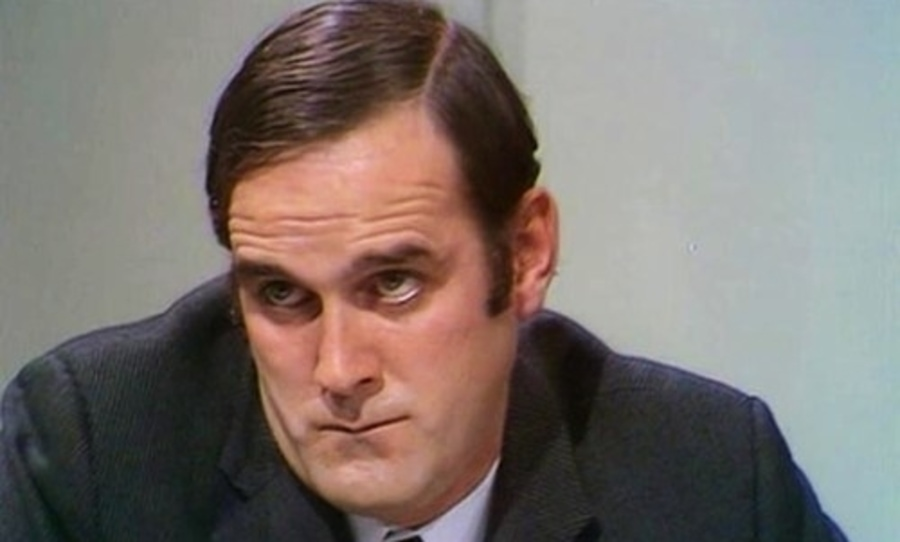
\includegraphics[width=1in,height=1.25in,clip,keepaspectratio]{monty1}}]{Jonathan Dorsey}
  I've already told you once. It is an ex parrot. Its has ceased to be. Recieved his Bachelors Degree in Mechanical Engineering from the San Jose State University. With a focus on mechatronics and control systems, he has developed an interest in reinforcement learning, computer vision, and control and design of autonomous systems.
\end{IEEEbiography}



\end{document}
